\documentclass{standalone}
\usepackage{tikz}
\usetikzlibrary{patterns, positioning}
\usepackage[sfdefault]{ClearSans} %% option 'sfdefault' activates Clear Sans as the default text font
\usepackage[T1]{fontenc}

\begin{document}
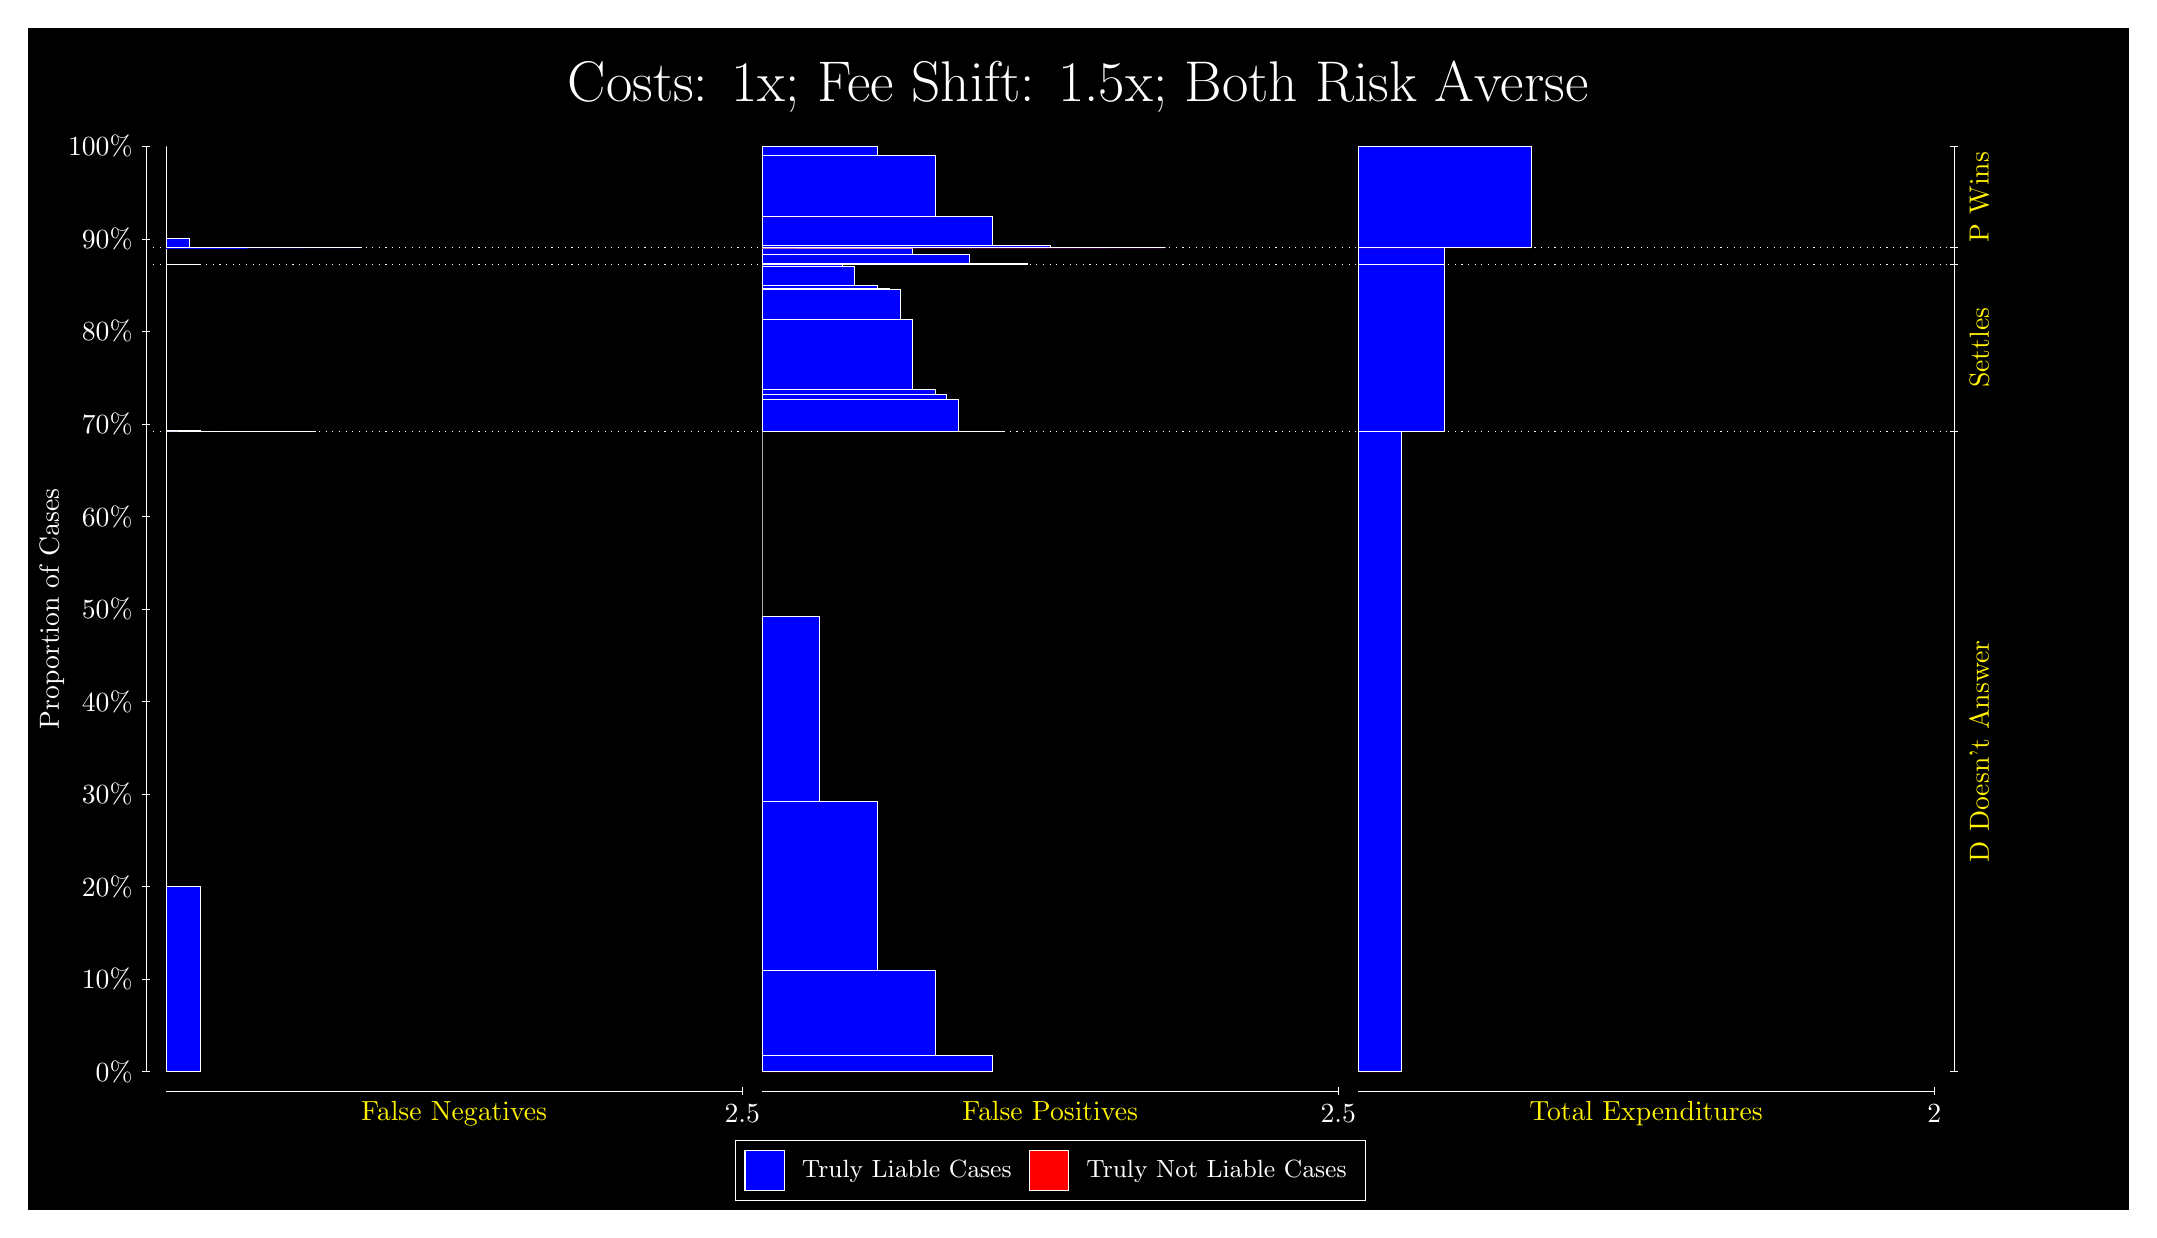
\begin{tikzpicture}
\draw[fill=black] (0,0) rectangle (26.667,15);
\draw[text=white] (0,13.5) rectangle (26.667,15) node[midway] {\huge Costs: 1x; Fee Shift: 1.5x; Both Risk Averse};
\draw[white, very thin] (1.5,1.75) -- (1.5,13.5);
\node[rotate=90, text=white, anchor=center] at (0.3, 7.625) {Proportion of Cases};
\draw[white, very thin] (1.45,1.75) -- (1.55,1.75);
\node[text=white, anchor=east] at (1.45, 1.75) {0\%};
\draw[white, very thin] (1.45,2.925) -- (1.55,2.925);
\node[text=white, anchor=east] at (1.45, 2.925) {10\%};
\draw[white, very thin] (1.45,4.1) -- (1.55,4.1);
\node[text=white, anchor=east] at (1.45, 4.1) {20\%};
\draw[white, very thin] (1.45,5.275) -- (1.55,5.275);
\node[text=white, anchor=east] at (1.45, 5.275) {30\%};
\draw[white, very thin] (1.45,6.45) -- (1.55,6.45);
\node[text=white, anchor=east] at (1.45, 6.45) {40\%};
\draw[white, very thin] (1.45,7.625) -- (1.55,7.625);
\node[text=white, anchor=east] at (1.45, 7.625) {50\%};
\draw[white, very thin] (1.45,8.8) -- (1.55,8.8);
\node[text=white, anchor=east] at (1.45, 8.8) {60\%};
\draw[white, very thin] (1.45,9.975) -- (1.55,9.975);
\node[text=white, anchor=east] at (1.45, 9.975) {70\%};
\draw[white, very thin] (1.45,11.15) -- (1.55,11.15);
\node[text=white, anchor=east] at (1.45, 11.15) {80\%};
\draw[white, very thin] (1.45,12.325) -- (1.55,12.325);
\node[text=white, anchor=east] at (1.45, 12.325) {90\%};
\draw[white, very thin] (1.45,13.5) -- (1.55,13.5);
\node[text=white, anchor=east] at (1.45, 13.5) {100\%};

\draw[white, very thin] (24.457,1.75) -- (24.457,13.5);
\draw[white, very thin] (24.407,1.75) -- (24.507,1.75);
\node[anchor=west] at (24.407, 1.75) {};
\draw[white, very thin] (24.407,9.8826) -- (24.507,9.8826);
\node[anchor=west] at (24.407, 9.8826) {};
\draw[white, very thin] (24.407,12.004) -- (24.507,12.004);
\node[anchor=west] at (24.407, 12.004) {};
\draw[white, very thin] (24.407,12.212) -- (24.507,12.212);
\node[anchor=west] at (24.407, 12.212) {};
\draw[white, very thin] (24.407,13.5) -- (24.507,13.5);
\node[anchor=west] at (24.407, 13.5) {};

\draw[white, very thin, fill=blue] (1.75,1.75) rectangle (2.1891,4.0999);
\draw[white, very thin, fill=red] (1.75,4.0999) rectangle (1.75,4.0999);
\draw[white, very thin, fill=blue] (1.75,4.0999) rectangle (1.75,9.8826);
\draw[white, very thin, fill=blue] (1.75,9.8826) rectangle (3.6529,9.8826);
\draw[white, very thin, fill=blue] (1.75,9.8826) rectangle (3.3602,9.8826);
\draw[white, very thin, fill=blue] (1.75,9.8826) rectangle (3.0674,9.8826);
\draw[white, very thin, fill=blue] (1.75,9.8826) rectangle (2.921,9.8826);
\draw[white, very thin, fill=blue] (1.75,9.8826) rectangle (2.6283,9.8826);
\draw[white, very thin, fill=blue] (1.75,9.8826) rectangle (2.4819,9.8826);
\draw[white, very thin, fill=blue] (1.75,9.8826) rectangle (2.3355,9.8826);
\draw[white, very thin, fill=blue] (1.75,9.8826) rectangle (2.1891,9.8899);
\draw[white, very thin, fill=blue] (1.75,9.8899) rectangle (1.8964,9.89);
\draw[white, very thin, fill=red] (1.75,9.89) rectangle (1.75,9.89);
\draw[white, very thin, fill=blue] (1.75,9.89) rectangle (1.75,12.004);
\draw[white, very thin, fill=blue] (1.75,12.004) rectangle (2.1891,12.004);
\draw[white, very thin, fill=red] (1.75,12.004) rectangle (1.75,12.004);
\draw[white, very thin, fill=blue] (1.75,12.004) rectangle (1.75,12.212);
\draw[white, very thin, fill=blue] (1.75,12.212) rectangle (4.2384,12.212);
\draw[white, very thin, fill=blue] (1.75,12.212) rectangle (3.5065,12.212);
\draw[white, very thin, fill=blue] (1.75,12.212) rectangle (2.7746,12.212);
\draw[white, very thin, fill=blue] (1.75,12.212) rectangle (2.7746,12.214);
\draw[white, very thin, fill=blue] (1.75,12.214) rectangle (2.0428,12.214);
\draw[white, very thin, fill=blue] (1.75,12.214) rectangle (2.0428,12.331);
\draw[white, very thin, fill=red] (1.75,12.331) rectangle (1.75,12.331);
\draw[white, very thin, fill=blue] (1.75,12.331) rectangle (1.75,13.5);
\draw[white, very thin, fill=red] (9.3189,1.75) rectangle (12.246,1.75);
\draw[white, very thin, fill=blue] (9.3189,1.75) rectangle (12.246,1.9502);
\draw[white, very thin, fill=blue] (9.3189,1.9502) rectangle (11.515,3.0419);
\draw[white, very thin, fill=blue] (9.3189,3.0419) rectangle (10.783,5.1844);
\draw[white, very thin, fill=blue] (9.3189,5.1844) rectangle (10.051,7.5326);
\draw[white, very thin, fill=blue] (9.3189,7.5326) rectangle (9.3189,9.8826);
\draw[white, very thin, fill=red] (9.3189,9.8826) rectangle (12.393,9.8826);
\draw[white, very thin, fill=blue] (9.3189,9.8826) rectangle (12.393,9.8866);
\draw[white, very thin, fill=red] (9.3189,9.8866) rectangle (11.807,9.8866);
\draw[white, very thin, fill=blue] (9.3189,9.8866) rectangle (11.807,10.288);
\draw[white, very thin, fill=blue] (9.3189,10.288) rectangle (11.661,10.355);
\draw[white, very thin, fill=red] (9.3189,10.355) rectangle (11.515,10.355);
\draw[white, very thin, fill=blue] (9.3189,10.355) rectangle (11.515,10.414);
\draw[white, very thin, fill=red] (9.3189,10.414) rectangle (11.222,10.414);
\draw[white, very thin, fill=blue] (9.3189,10.414) rectangle (11.222,11.306);
\draw[white, very thin, fill=blue] (9.3189,11.306) rectangle (11.075,11.679);
\draw[white, very thin, fill=blue] (9.3189,11.679) rectangle (10.929,11.698);
\draw[white, very thin, fill=blue] (9.3189,11.698) rectangle (10.783,11.74);
\draw[white, very thin, fill=blue] (9.3189,11.74) rectangle (10.49,11.982);
\draw[white, very thin, fill=blue] (9.3189,11.982) rectangle (10.344,11.997);
\draw[white, very thin, fill=blue] (9.3189,11.997) rectangle (10.197,11.997);
\draw[white, very thin, fill=blue] (9.3189,11.997) rectangle (10.051,11.997);
\draw[white, very thin, fill=blue] (9.3189,11.997) rectangle (9.758,12.004);
\draw[white, very thin, fill=blue] (9.3189,12.004) rectangle (9.6116,12.004);
\draw[white, very thin, fill=blue] (9.3189,12.004) rectangle (9.4652,12.004);
\draw[white, very thin, fill=blue] (9.3189,12.004) rectangle (9.3189,12.004);
\draw[white, very thin, fill=red] (9.3189,12.004) rectangle (12.686,12.004);
\draw[white, very thin, fill=blue] (9.3189,12.004) rectangle (12.686,12.009);
\draw[white, very thin, fill=blue] (9.3189,12.009) rectangle (11.954,12.135);
\draw[white, very thin, fill=blue] (9.3189,12.135) rectangle (11.222,12.211);
\draw[white, very thin, fill=blue] (9.3189,12.211) rectangle (10.49,12.212);
\draw[white, very thin, fill=blue] (9.3189,12.212) rectangle (9.758,12.212);
\draw[white, very thin, fill=red] (9.3189,12.212) rectangle (14.442,12.212);
\draw[white, very thin, fill=blue] (9.3189,12.212) rectangle (14.442,12.212);
\draw[white, very thin, fill=red] (9.3189,12.212) rectangle (13.71,12.212);
\draw[white, very thin, fill=blue] (9.3189,12.212) rectangle (13.71,12.212);
\draw[white, very thin, fill=red] (9.3189,12.212) rectangle (12.978,12.212);
\draw[white, very thin, fill=blue] (9.3189,12.212) rectangle (12.978,12.247);
\draw[white, very thin, fill=red] (9.3189,12.247) rectangle (12.246,12.247);
\draw[white, very thin, fill=blue] (9.3189,12.247) rectangle (12.246,12.606);
\draw[white, very thin, fill=red] (9.3189,12.606) rectangle (11.515,12.606);
\draw[white, very thin, fill=blue] (9.3189,12.606) rectangle (11.515,13.381);
\draw[white, very thin, fill=blue] (9.3189,13.381) rectangle (10.783,13.498);
\draw[white, very thin, fill=blue] (9.3189,13.498) rectangle (10.051,13.5);
\draw[white, very thin, fill=blue] (9.3189,13.5) rectangle (9.3189,13.5);
\draw[white, very thin, fill=red] (16.888,1.75) rectangle (17.437,1.75);
\draw[white, very thin, fill=blue] (16.888,1.75) rectangle (17.437,9.8826);
\draw[white, very thin, fill=red] (16.888,9.8826) rectangle (17.986,9.8826);
\draw[white, very thin, fill=blue] (16.888,9.8826) rectangle (17.986,12.004);
\draw[white, very thin, fill=red] (16.888,12.004) rectangle (17.986,12.004);
\draw[white, very thin, fill=blue] (16.888,12.004) rectangle (17.986,12.212);
\draw[white, very thin, fill=red] (16.888,12.212) rectangle (19.083,12.212);
\draw[white, very thin, fill=blue] (16.888,12.212) rectangle (19.083,13.5);
\draw[white, dotted] (1.5,9.8826) -- (24.457,9.8826);
\draw[white, dotted] (1.5,12.004) -- (24.457,12.004);
\draw[white, dotted] (1.5,12.212) -- (24.457,12.212);
\draw[white, very thin] (1.75,1.5) -- (9.0689,1.5);
\node[text=yellow, anchor=north] at (5.4094, 1.5) {False Negatives};
\draw[white, very thin] (9.0689,1.45) -- (9.0689,1.55);
\node[text=white, anchor=north] at (9.0689, 1.45) {2.5};

\draw[white, very thin] (9.3189,1.5) -- (16.638,1.5);
\node[text=yellow, anchor=north] at (12.978, 1.5) {False Positives};
\draw[white, very thin] (16.638,1.45) -- (16.638,1.55);
\node[text=white, anchor=north] at (16.638, 1.45) {2.5};

\draw[white, very thin] (16.888,1.5) -- (24.207,1.5);
\node[text=yellow, anchor=north] at (20.547, 1.5) {Total Expenditures};
\draw[white, very thin] (24.207,1.45) -- (24.207,1.55);
\node[text=white, anchor=north] at (24.207, 1.45) {2};

\node[text=yellow, centered, rotate=90] at (24.777, 5.8163) {D Doesn't Answer};
\node[text=yellow, centered, rotate=90] at (24.777, 10.943) {Settles};

\node[text=yellow, centered, rotate=90] at (24.777, 12.856) {P Wins};

\draw (12.978300999999998,1.5) node[draw=none] (baseCoordinate) {};
\begin{scope}[align=center]
        \matrix[scale=0.5, draw=white, below=0.5cm of baseCoordinate, nodes={draw}, column sep=0.1cm]{
            \node[rectangle, draw, minimum width=0.5cm, minimum height=0.5cm, fill=blue] {}; &
            \node[draw=none, font=\small, text=white] (B) {Truly Liable Cases}; &
            \node[rectangle, draw, minimum width=0.5cm, minimum height=0.5cm, fill=red] {}; &
            \node[draw=none, font=\small, text=white] (B) {Truly Not Liable Cases}; \\
            };
\end{scope}

\end{tikzpicture}
\end{document}